\section{Radiography}
Radiography is the simplest form of medical imaging based on X-rays. These rays
can travel through solid objects, but attenuate depending on the materials they
meet along their path. For example, when passing through a human hand, the
attenuation is stronger when passing through bones rather than through soft
tissue. The image can be recorded (in negative) on ordinary photographic paper
and processed in darkrooms. \autoref{fig:xrayhand} shows am example.

\begin{figure}[ht]
\begin{center}
  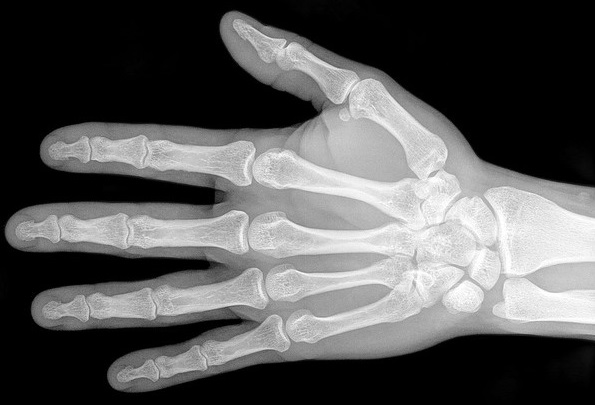
\includegraphics[width=\linewidth]{img/xrayhand.jpg}
  \caption{X-ray image of a human hand. In this negative image, bones are
  lighter because fewer X-rays managed to get through them.}
  \label{fig:xrayhand}
\end{center}
\end{figure}

\subsection{History}
Radiography builds on the work of Wilhelm Konrad R\"ontgen, a German physicist
who produced and detected X-rays for the first time on November 8, 1895.
These X-rays (X for unknown) had the remarkable property of being attenuated at
different rates when passing through various materials. For example, bone
strongly attenuates the X-rays while soft tissue does much less so. R\"ontgen
also discovered that the radiation can be captured on a photographic plate, just
like regular light. He presented his findings in his paper ``On a new kind or
rays'' \cite{rontgen}. This discovery earned him the Nobel Prize in Physics in
1901.

Only two weeks after his discovery he produced the first X-ray photo of his
wife's hand, after which she reportedly exclaimed: ``I have seen my death!''.
Just a couple of months later, X-rays were already being used in a clinical
setting on patients.

Note that during this time, not much was known about ionizing radiation or
radioactivity. Only a year after the discovery of X-rays did Henri Becquerel
discover radioactivity. Well known scientists such as Ernest Rutherford and
Pierre \& Marie Curie performed several more years worth of research before
realizing the true danger of prolonged exposure to this type of radiation.

\subsection{Technical background}
To better understand the internal workings of imaging devices, we present a
simplified mathematical and physical background based on the book of prof.
Suetens\cite{suetens}. X-rays are simply a form of electromagnetic waves
consisting of photons with a wavelength $\lambda$ on the order of Angstr\o ms
($10^{-10}$m). The corresponding frequency $f$ places these rays firmly in the
ionizing part of the spectrum - that is, they can cause cancer.
\autoref{fig:spectrum} shows a schematic overview of the whole spectrum. The
energy of such a wave can be calculated with the following formula, where $c$
is the speed of light and $h$ is Planck's constant.

\begin{figure}[ht]
\begin{center}
  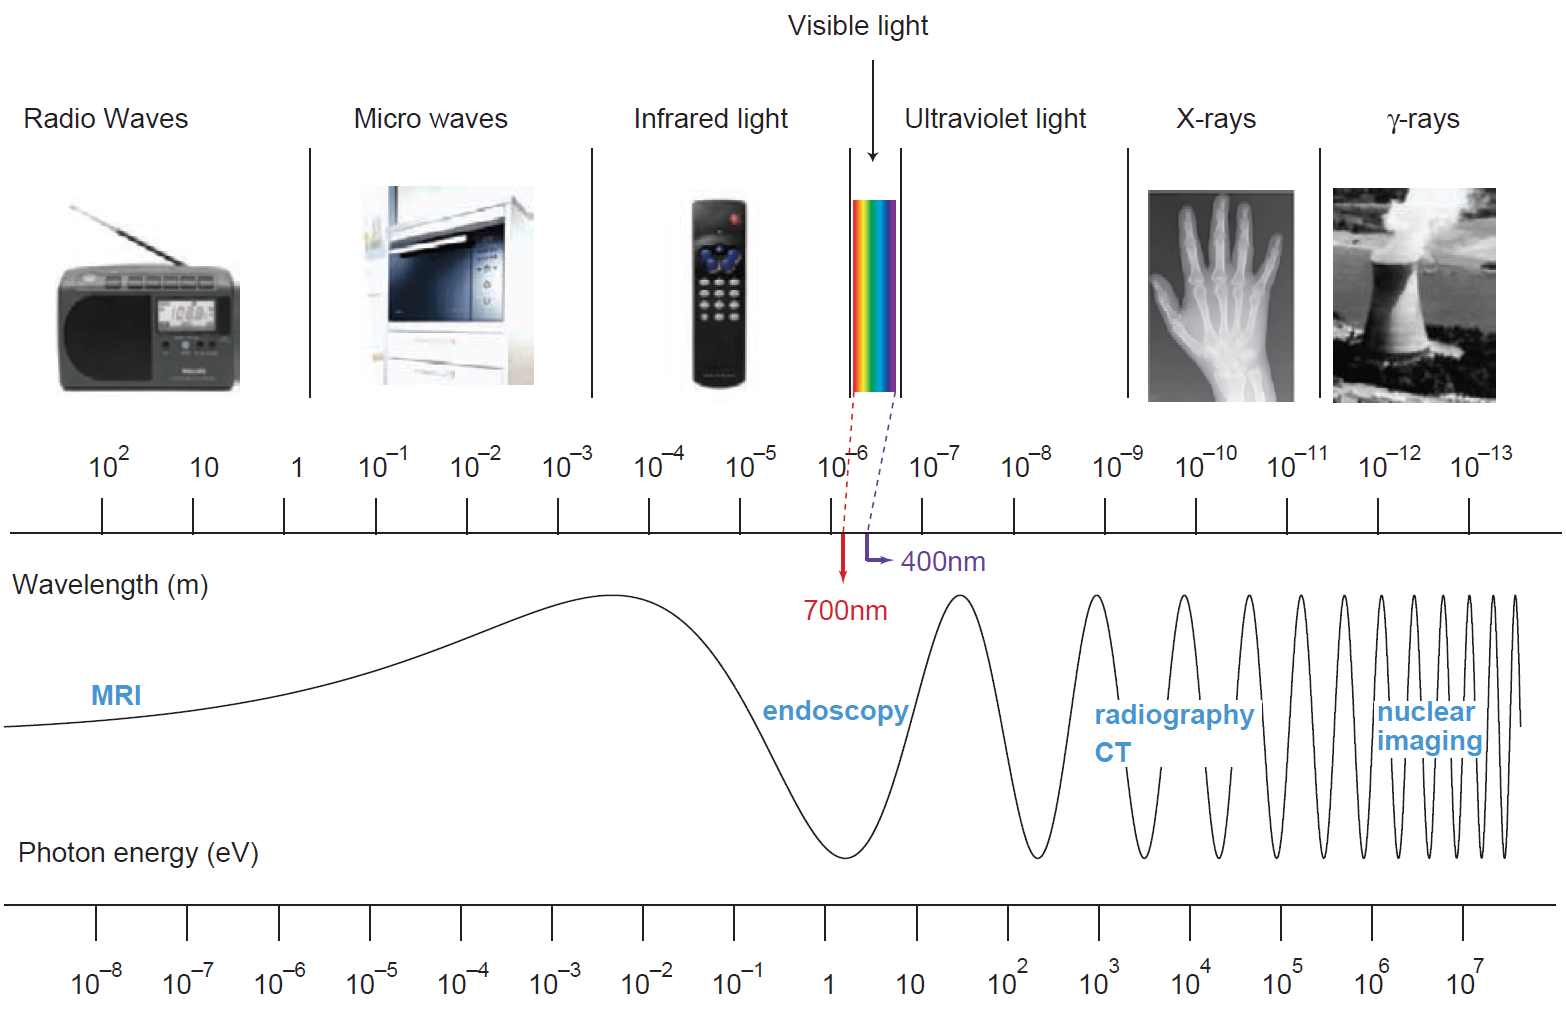
\includegraphics[width=\linewidth]{img/spectrum.png}
  \caption{The electromagnetic spectrum. \cite{suetens}}
  \label{fig:spectrum}
\end{center}
\end{figure}

\begin{equation}
	E = hf = \frac{hc}{\lambda}.
\end{equation}

X-rays are generated in an X-ray tube, a vacuum tube consisting of a cathode and
an anode. Current flowing through the cathode releases electrons,
which are accelerated toward the anode by an applied voltage. Once the electrons
hit the anode, they release part of their energy in the form of X-ray photons.
Thus, the two most important settings of an X-ray scan are the applied
current multiplied by the exposure time (mA $\cdot$ s) and the applied voltage
(keV).

The attenuation of X-rays through materials can easily be modeled using an
attenuation coefficient $\mu$. The beam intensity when passed through a
homogeneous material of depth $d$ is given by: 

\begin{equation}
	I_{out} = I_{in} \cdot \exp (-\mu d).
\end{equation}

This formula can of course easily be extended to include heterogeneous materials
and variable attenuation coefficients.

To capture X-rays, a detector is needed. Traditionally, a screen-film detector
was used. The familiar photographic film alone is very inefficient
at capturing X-rays: only about 2\% of all photons are absorbed. Because X-rays
are ionizing, the applied dose cannot simply be increased to improve the
image quality. Instead, an intensifier screen is used in front of the film. This
screen contains heavy chemical elements, whose electrons are excited by the
incoming photons. When returning to their original state, these electrons emit
visible light that can be captured more efficiently by the film, raising the
absorption rate to about 50\%.

Besides ordinary radiography, special classes such as fluoroscopy and
mammography exist. Fluoroscopy generates time-lapse recordings instead of still
images. With modern technology, tens of frames per second are achievable. Of
course, each frame must be shot at a very low exposure rate to minimize patient
risk. Mammography on the other hand produces images of the human breast. The
challenge here is to generate very high resolution images, so that small masses
can be seen.

\subsection{Recent advancements}\label{ssec:recentradio}
Relatively recently, X-ray systems have moved away from analogue detectors
towards digital ones. Much like digital photographs, digital X-ray scans are far
easier to store, copy, post-process and share. On top of that, they typically
have a much wider exposure range making them more tolerant to over- and
underexposure. These detector systems use storage phosphors to temporarily hold
the absorbed radiation instead of immediately releasing it in the form of
photons. This phenomenon is caused by electron traps in the doped material.
Later, this phosphor can be read out pixel-wise using an optical detector array
and a laser that gives the electrons enough energy to escape their trap. The
main obstacle for this paradigm shift was the large pixel size. Large pixels
translate to lower resolution, which is turn leads to a loss of diagnostic
value. Only by the time pixels could be as small as 0.1 mm did the medical world
embrace digital detectors \cite{review}.

Even newer devices use active matrix flat panel detectors. These detectors are
able to produce near real time images. In comparison, storage phosphors and
older technologies required minutes or more of processing time.

\subsubsection{A note on image quality}\label{sssec:imgquality}
The quality of an image can be expressed in three dimensions: resolution,
contrast and noise \cite{suetens}.

Resolution is sometimes simply stated as the pixel density (dots per inch).
However, this only provides an upper bound because in practise neighbouring
pixels are often correlated. For example, due to the imperfect nature of the
recording equipment, a single point can appear as blurred blob on the resulting
image. This blob is called the Point Spread Function (PSF), and is a better
measure for the actual image resolution. If the resolution is isotropic, the
Line Spread Function (LSF) - measured in distinguishable line pairs per
millimeter (lp/mm) - can also be used. Alternatively, the Optical Transfer
Function (OTF, sometimes also called MTF) representing amplitude and phase
shifts of a sinusoidal target can be used. In fact, this OTF is nothing more than the
Fourier transform of the PSF or LSF.

Second, contrast is the intensity difference between neighbouring regions of the
image. More formally, contrast at a given frequency is the amplitude component
of the image at that frequency in the frequency domain (calculated using the
Fourier transform). Contrast is dependent on the whole imaging process, but also
on the size and shape of the objects in the image. 

Third, noise is partly the result of interfering phenomena. Yet, it is also
inherent to the electromagnetic radiation itself because the waves themselves
are stochastic processes. An important measure is the Signal to Noise Ratio
(SNR) or, more appropriately, the Contrast to Noise Ratio (CNR). Noise can be
estimated by examining the result of an scan with no object present, a so-called
flat-field image. Another measure for the amount of noise is the Wiener
spectrum.

Another frequently used metric called the Detective Quantum Efficiency (DQE) can
compare various technologies without being dependent on the object being imaged.

\begin{equation}
DQE(f) = \frac{SNR(f)_{out}^2}{SNR(f)_{in}^2}
\end{equation}

In addition to these elements, sometimes artifacts appear on scans. The
causes of these artificial image features vary widely depending on the image
modality used and can also be caused by excessive post-processing.

\subsection{Future expectations}
Ever since CT scanners - and to a lesser extent MRI scanners - made their way
into hospitals, they have taken over many of the tasks traditionally reserved
for basic radiography. This declining trend is expected to continue in the
foreseeable future.